\documentclass[]{article}
\usepackage{lmodern}
\usepackage{amssymb,amsmath}
\usepackage{ifxetex,ifluatex}
\usepackage{fixltx2e} % provides \textsubscript
\ifnum 0\ifxetex 1\fi\ifluatex 1\fi=0 % if pdftex
  \usepackage[T1]{fontenc}
  \usepackage[utf8]{inputenc}
\else % if luatex or xelatex
  \ifxetex
    \usepackage{mathspec}
  \else
    \usepackage{fontspec}
  \fi
  \defaultfontfeatures{Ligatures=TeX,Scale=MatchLowercase}
\fi
% use upquote if available, for straight quotes in verbatim environments
\IfFileExists{upquote.sty}{\usepackage{upquote}}{}
% use microtype if available
\IfFileExists{microtype.sty}{%
\usepackage{microtype}
\UseMicrotypeSet[protrusion]{basicmath} % disable protrusion for tt fonts
}{}
\usepackage[margin=1in]{geometry}
\usepackage{hyperref}
\hypersetup{unicode=true,
            pdftitle={R: manipulación de datos},
            pdfborder={0 0 0},
            breaklinks=true}
\urlstyle{same}  % don't use monospace font for urls
\usepackage{color}
\usepackage{fancyvrb}
\newcommand{\VerbBar}{|}
\newcommand{\VERB}{\Verb[commandchars=\\\{\}]}
\DefineVerbatimEnvironment{Highlighting}{Verbatim}{commandchars=\\\{\}}
% Add ',fontsize=\small' for more characters per line
\usepackage{framed}
\definecolor{shadecolor}{RGB}{248,248,248}
\newenvironment{Shaded}{\begin{snugshade}}{\end{snugshade}}
\newcommand{\KeywordTok}[1]{\textcolor[rgb]{0.13,0.29,0.53}{\textbf{#1}}}
\newcommand{\DataTypeTok}[1]{\textcolor[rgb]{0.13,0.29,0.53}{#1}}
\newcommand{\DecValTok}[1]{\textcolor[rgb]{0.00,0.00,0.81}{#1}}
\newcommand{\BaseNTok}[1]{\textcolor[rgb]{0.00,0.00,0.81}{#1}}
\newcommand{\FloatTok}[1]{\textcolor[rgb]{0.00,0.00,0.81}{#1}}
\newcommand{\ConstantTok}[1]{\textcolor[rgb]{0.00,0.00,0.00}{#1}}
\newcommand{\CharTok}[1]{\textcolor[rgb]{0.31,0.60,0.02}{#1}}
\newcommand{\SpecialCharTok}[1]{\textcolor[rgb]{0.00,0.00,0.00}{#1}}
\newcommand{\StringTok}[1]{\textcolor[rgb]{0.31,0.60,0.02}{#1}}
\newcommand{\VerbatimStringTok}[1]{\textcolor[rgb]{0.31,0.60,0.02}{#1}}
\newcommand{\SpecialStringTok}[1]{\textcolor[rgb]{0.31,0.60,0.02}{#1}}
\newcommand{\ImportTok}[1]{#1}
\newcommand{\CommentTok}[1]{\textcolor[rgb]{0.56,0.35,0.01}{\textit{#1}}}
\newcommand{\DocumentationTok}[1]{\textcolor[rgb]{0.56,0.35,0.01}{\textbf{\textit{#1}}}}
\newcommand{\AnnotationTok}[1]{\textcolor[rgb]{0.56,0.35,0.01}{\textbf{\textit{#1}}}}
\newcommand{\CommentVarTok}[1]{\textcolor[rgb]{0.56,0.35,0.01}{\textbf{\textit{#1}}}}
\newcommand{\OtherTok}[1]{\textcolor[rgb]{0.56,0.35,0.01}{#1}}
\newcommand{\FunctionTok}[1]{\textcolor[rgb]{0.00,0.00,0.00}{#1}}
\newcommand{\VariableTok}[1]{\textcolor[rgb]{0.00,0.00,0.00}{#1}}
\newcommand{\ControlFlowTok}[1]{\textcolor[rgb]{0.13,0.29,0.53}{\textbf{#1}}}
\newcommand{\OperatorTok}[1]{\textcolor[rgb]{0.81,0.36,0.00}{\textbf{#1}}}
\newcommand{\BuiltInTok}[1]{#1}
\newcommand{\ExtensionTok}[1]{#1}
\newcommand{\PreprocessorTok}[1]{\textcolor[rgb]{0.56,0.35,0.01}{\textit{#1}}}
\newcommand{\AttributeTok}[1]{\textcolor[rgb]{0.77,0.63,0.00}{#1}}
\newcommand{\RegionMarkerTok}[1]{#1}
\newcommand{\InformationTok}[1]{\textcolor[rgb]{0.56,0.35,0.01}{\textbf{\textit{#1}}}}
\newcommand{\WarningTok}[1]{\textcolor[rgb]{0.56,0.35,0.01}{\textbf{\textit{#1}}}}
\newcommand{\AlertTok}[1]{\textcolor[rgb]{0.94,0.16,0.16}{#1}}
\newcommand{\ErrorTok}[1]{\textcolor[rgb]{0.64,0.00,0.00}{\textbf{#1}}}
\newcommand{\NormalTok}[1]{#1}
\usepackage{graphicx,grffile}
\makeatletter
\def\maxwidth{\ifdim\Gin@nat@width>\linewidth\linewidth\else\Gin@nat@width\fi}
\def\maxheight{\ifdim\Gin@nat@height>\textheight\textheight\else\Gin@nat@height\fi}
\makeatother
% Scale images if necessary, so that they will not overflow the page
% margins by default, and it is still possible to overwrite the defaults
% using explicit options in \includegraphics[width, height, ...]{}
\setkeys{Gin}{width=\maxwidth,height=\maxheight,keepaspectratio}
\IfFileExists{parskip.sty}{%
\usepackage{parskip}
}{% else
\setlength{\parindent}{0pt}
\setlength{\parskip}{6pt plus 2pt minus 1pt}
}
\setlength{\emergencystretch}{3em}  % prevent overfull lines
\providecommand{\tightlist}{%
  \setlength{\itemsep}{0pt}\setlength{\parskip}{0pt}}
\setcounter{secnumdepth}{0}
% Redefines (sub)paragraphs to behave more like sections
\ifx\paragraph\undefined\else
\let\oldparagraph\paragraph
\renewcommand{\paragraph}[1]{\oldparagraph{#1}\mbox{}}
\fi
\ifx\subparagraph\undefined\else
\let\oldsubparagraph\subparagraph
\renewcommand{\subparagraph}[1]{\oldsubparagraph{#1}\mbox{}}
\fi

%%% Use protect on footnotes to avoid problems with footnotes in titles
\let\rmarkdownfootnote\footnote%
\def\footnote{\protect\rmarkdownfootnote}

%%% Change title format to be more compact
\usepackage{titling}

% Create subtitle command for use in maketitle
\newcommand{\subtitle}[1]{
  \posttitle{
    \begin{center}\large#1\end{center}
    }
}

\setlength{\droptitle}{-2em}
  \title{R: manipulación de datos}
  \pretitle{\vspace{\droptitle}\centering\huge}
  \posttitle{\par}
  \author{}
  \preauthor{}\postauthor{}
  \date{}
  \predate{}\postdate{}

\usepackage[
  backend=biber,
  style=alphabetic,
  sorting=ynt,
  citestyle=authoryear
  ]{biblatex}
\addbibresource{../lit/bib.bib}

\usepackage[utf8]{inputenc}
\usepackage[spanish]{babel}
\usepackage{float}
%%%% Frames
\ifxetex
    \makeatletter % undo the wrong changes made by mathspec
    \let\RequirePackage\original@RequirePackage
    \let\usepackage\RequirePackage
    \makeatother
\fi

\usepackage{xcolor}
\usepackage[tikz]{bclogo}
\usepackage[framemethod=tikz]{mdframed}
\usepackage{lipsum}
\usepackage[many]{tcolorbox}

\definecolor{bgblue}{RGB}{245,243,253}
\definecolor{ttblue}{RGB}{91,194,224}
\definecolor{llred}{RGB}{255,228,225}
\definecolor{bbblack}{RGB}{0,0,0}

\mdfdefinestyle{mystyle}{%
  rightline=true,
  innerleftmargin=10,
  innerrightmargin=10,
  outerlinewidth=3pt,
  topline=false,
  rightline=true,
  bottomline=false,
  skipabove=\topsep,
  skipbelow=\topsep
}

\newtcolorbox{curiosidad}[1][]{
  breakable,
  title=#1,
  colback=white,
  colbacktitle=white,
  coltitle=black,
  fonttitle=\bfseries,
  bottomrule=0pt,
  toprule=0pt,
  leftrule=3pt,
  rightrule=3pt,
  titlerule=0pt,
  arc=0pt,
  outer arc=0pt,
  colframe=black,
}

\newtcolorbox{nota}[1][]{
  breakable,
  freelance,
  title=#1,
  colback=white,
  colbacktitle=white,
  coltitle=black,
  fonttitle=\bfseries,
  bottomrule=0pt,
  boxrule=0pt,
  colframe=white,
  overlay unbroken and first={
  \draw[red!75!black,line width=3pt]
    ([xshift=5pt]frame.north west) -- 
    (frame.north west) -- 
    (frame.south west);
  \draw[red!75!black,line width=3pt]
    ([xshift=-5pt]frame.north east) -- 
    (frame.north east) -- 
    (frame.south east);
  },
  overlay unbroken app={
  \draw[red!75!black,line width=3pt,line cap=rect]
    (frame.south west) -- 
    ([xshift=5pt]frame.south west);
  \draw[red!75!black,line width=3pt,line cap=rect]
    (frame.south east) -- 
    ([xshift=-5pt]frame.south east);
  },
  overlay middle and last={
  \draw[red!75!black,line width=3pt]
    (frame.north west) -- 
    (frame.south west);
  \draw[red!75!black,line width=3pt]
    (frame.north east) -- 
    (frame.south east);
  },
  overlay last app={
  \draw[red!75!black,line width=3pt,line cap=rect]
    (frame.south west) --
    ([xshift=5pt]frame.south west);
  \draw[red!75!black,line width=3pt,line cap=rect]
    (frame.south east) --
    ([xshift=-5pt]frame.south east);
  },
}

\begin{document}
\maketitle

\section{Manipulación de datos}\label{manipulacion-de-datos}

Esta sección resume algunas de las funciones existentes para
\textbf{limpiar} datos de distintos formatos a \texttt{R}. En
particular, se utiliza la conceptualización de datos limpios presentada
en \textcite{wickham2014tidy} e implementada en el paquete
\texttt{tidyr} \parencite{tidyr}. En la figura \ref{fig:ciclo2} podemos
ver la etapa del análisis de datos correspondiente.

\begin{figure}[h]
    \centering
    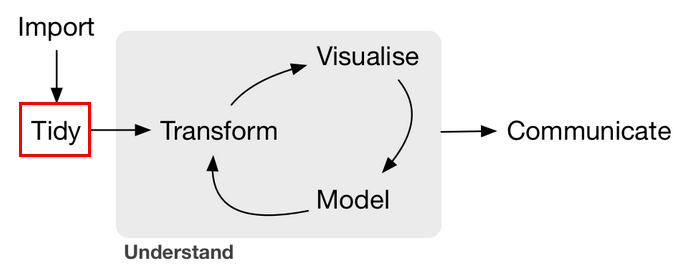
\includegraphics[width=0.75\textwidth]{../img/02_ciclo_2.png}
    \caption{Limpieza de datos \textcite[Introducción]{grolemund2016r}.}
    \label{fig:ciclo2}
\end{figure}

\subsection{Datos limpios}\label{datos-limpios}

Mucho del esfuerzo en analítica lidia con la limpieza de datos. Tomar
datos de diferentes fuentes y poderlas poner en la forma en la que uno
los necesita para realizar analítica toma mucho tiempo y esfuerzo.
Existen herramientas que permiten que esta parte sea más fácil y
eficiente. Entre éstas se encuentran los criterios de datos limpios.

Los conjuntos de datos limpios (\emph{tidy datasets}) permiten
manipularlos fácilmente, modelarlos y visualizarlos. Además, tienen una
estructura específica: cada variable es una columna, cada observación
una fila y cada tipo de unidad observacional es una tabla.

\subsubsection{Preparación de datos}\label{preparacion-de-datos}

Esta actividad incluye una gran cantidad de elementos: desde revisar los
outliers, hasta extraer variables de cadenas en datos no estrucutrados,
imputación de valores perdidos. Los datos limpios son tan solo un
subconjunto de este proceso y lidian con el cómo estructurar los datos
de manera que se facilite el análisis.

El estándar de datos limpios está diseñado para facilitar la exploración
inicial y el análisis de datos así como simplificar el desarrollo de
herramientas para el análsis de datos que trabajen bien con datos
limpios.

Los criterios de datos limpios están muy relacionados a los de las bases
de datos relacionales y, por ende, al algebra relacional de Codd. Sin
embargo, se expresan y enmarcan en lenguaje que le es familiar a
estadísticos.

Básicamente, están creados para lidear con conjuntos de datos que se
encuentran en el mundo real. Los criterios de datos limpios proporcionan
un marco mental a través del cual la intuición es explícita.

\subsubsection{Definición de datos
limpios}\label{definicion-de-datos-limpios}

Los datos limpios proporcionan una manera estándar de ligar la
estructura de un dataset (es decir su layout físico) con su semántica
(su significado).

\subsubsection{Estructura de datos}\label{estructura-de-datos}

La mayoría de los datos estadísticos están conformados por tablas
rectangulares compuestas por filas y columnas. Las columnas casi siempre
están etiquetadas \emph{colnames} y las filas a veces lo están.

Tomamos el ejemplo de datos de la figura \ref{fig:estructura} en donde
se presentan datos de un experimento. La tabla contiene dos columas y
tres filas, ambas etiquetadas.

\begin{figure}[h]
    \centering
    \includegraphics[width=0.4\textwidth]{../img/02_estructura.png}
    \caption{Típica presentación de datos.}
    \label{fig:estructura}
\end{figure}

Podemos estructurar los datos de diferentes maneras pero la abstracción
de filas y columnas solamente nos permite pensar en la representación
transpuesta que se muestra en la figura \ref{fig:estructurat}. El layout
cambia pero los datos son los mismos. Con columnas y filas, no podemos
decir esto de manera apropiada. Además de la simple apariencia, debemos
poder describir la semántica -el significado- de los valores que se
muestran en una tabla.

\begin{figure}[h]
    \centering
    \includegraphics[width=0.5\textwidth]{../img/02_estructurat.png}
    \caption{Mismos datos que en \ref{fig:estructura} pero traspuestos.}
    \label{fig:estructurat}
\end{figure}

\subsubsection{Semántica}\label{semantica}

Un conjunto de datos es una colección de \textbf{valores} (normalmente
cuantitativos/números o cualitativos/caracteres).

Los valores se organian de dos maneras. Cada valor pertenece a una
variable y a una observación. Una variable contiene todos los valores de
una medida y del mismo atributo subyacente (por ejemplo, temperatura,
duración, altura, latitud) a través de unidades. Una observación, en
cambio, contiene todos los valores medidos para la misma unidad (por
ejemplo, una persona, un día, un municipio) a través de distintos
atributos.

Los mismos datos en las figuras \ref{fig:estructura} y
\ref{fig:estructurat} los pensamos ahora en estos términos. Tenemos 3
variables:

\begin{enumerate}
\def\labelenumi{\arabic{enumi}.}
\tightlist
\item
  \emph{persona} con tres posibles valores (John, Jane, Mary)
\item
  \emph{tratamiento} con dos posibles valores (a o b)
\item
  \emph{resultado} con 5 o 6 valores (-, 16, 3, 2, 11, 1)
\end{enumerate}

El diseño del experimento mismo nos habla de la estructura de las
observaciones y los posibles valores que pueden tomar. Por ejemplo, en
este caso el valor perdido nos dice que, por diseño, se debió de
capturar esta variable pero no se hizo (por eso es importante guardarlo
como tal). Los valores perdidos estructurales, representan mediciones de
valores que no se puede hacer o que no suceden y, por tanto, se pueden
eliminar (por ejemplo, hombres embarazados). En la figura
\ref{fig:estructuratidy} se muestran los mismos datos que antes pero
pensados tal que las variables son columnas y las observaciones (en este
caso, cada punto en el diseño experimental) son filas.

\begin{figure}[h]
    \centering
    \includegraphics[width=0.4\textwidth]{../img/02_estructuratidy.png}
    \caption{Observaciones son filas, variables columnas.}
    \label{fig:estructuratidy}
\end{figure}

Normalmente, es fácil determinar qué son observaciones y qué son
variables pero es muy dificil definir en forma precisa variables y
observaciones. Por ejemplo, si tienes teléfonos de casa y celulares, se
pueden considerar como dos variables distintas en muchos contextos pero
en prevención de fraude necesitas una variable que guarde el tipo de
teléfono y otra en la que se guarde el número pues el uso regular del
mismo número de teléfono por parte de la misma persona puede ayudar a
detectarlo.

En general, es más fácil describir las relaciones funcionales entre las
variables que entre las filas (el radio, una combinación lineal).
También es más fácil hacer comparaciones entre grupos que entre columnas
(la suma, el promedio, la varianza, la moda).

\subsubsection{Datos limpios}\label{datos-limpios-1}

Éstos mapean de forma estándar el significado y la estructura de los
datos. Un conjunto de datos se considera sucio o limpio dependendiendo
en cómo las filas, columans y tablas mapean a observaciones, variables y
tipos. En \textbf{datos limpios}:

\begin{enumerate}
\def\labelenumi{\arabic{enumi}.}
\tightlist
\item
  Cada \emph{variable} es una columna.
\item
  Cada \emph{observación} es una fila.
\item
  Cada \emph{tipo de unidad observacional} es una tabla.
\end{enumerate}

Esto equivale a la tercera forma normal de Codd enfocado a un solo
conjunto de datos y no a datos conectados como en bases relacionales.
Los datos sucios son cualquier otro tipo de manera de organizar los
datos.

La tabla \ref{fig:estructuratidy} corresponde a datos limpios: cada fila
es una observación, es decir, el resultado de un tratamiento a una
persona. Cada columna es una variable. Solo tenemos un tipo de unidad
observacional, es decir, cada renglón es una unidad del diseño
experimental.

Con los datos así ordenados, suele ser más fácil extraer datos que, por
ejemplo, la \ref{fig:estructura}.

\renewcommand\bcStyleTitre[1]{\large\textcolor{bbblack}{#1}}

\begin{bclogo}[
  couleur=llred,
  arrondi=0,
  logo=\bcstop,
  barre=none,
  noborder=true]{Ejercicios}
\begin{enumerate}
\item Crea un dataframe con los valores de la tabla \ref{fig:estructura} y otro 
con los valores de la tabla \ref{fig:estructuratidy}.
\item Extrae el resultado para John Smith, tratamiento a en la primera configuración y en la segunda.
\item Especifica el número de tratamientos con la forma sucia y la forma limpia.
\item ¿Cuál es la media de los resultados? Usa la forma 1 y la forma 2.
\item Extrae los tratamientos del tipo a en la forma 2.
\end{enumerate}

\end{bclogo}

Como puedes ver, los datos limpios nos permiten preguntarle cosas a los
datos de manera simple y sistemática. En particular, es una estructura
muy útil para programación vectorizada como en R (el ejercicio 5) porque
la forma se asegura que valores para diferentes variables de la misma
observación siempre están apareados.

Por convención, las variables se acomodan de una forma particular. Las
variables \emph{fijas}, en este ejemplo, las propias al diseño
experimental, van primero y posteriormente las variables \emph{medidas}.
Ordenamos éstas de forma que las que están relacionadas sean contiguas.

\subsection{De sucio a limpio}\label{de-sucio-a-limpio}

Los conjuntos de datos normalmente \textbf{no cumplen} con estos
criterios. Es raro obtener un conjunto de datos con el cuál podemos
trabajar de manera inmediata.

Los 5 problemas más comunes para llevar datos sucios a limpios son

\begin{enumerate}
\def\labelenumi{\arabic{enumi}.}
\tightlist
\item
  Los nombres de las columnas son valores, no nombres de variables.
\item
  Múltiples variables se encuentran en la misma columna.
\item
  Las variables están guardadas tanto en filas como en columnas.
\item
  Muchos tipos de unidad observacional se encuentran en la misma tabla.
\item
  Una sola unidad observarcional se guardó en varias tablas.
\end{enumerate}

Estos problemas pueden ser resueltos con 3 herramientas: \emph{melting},
separación de cadenas y \emph{casting}.

\subsubsection{Los nombres de las columnas son valores, no nombres de
variables}\label{los-nombres-de-las-columnas-son-valores-no-nombres-de-variables}

La tabla \ref{tab:varsencols} muestra datos sucios con este problema. La
base acompaña al paquete \texttt{tidyr} {[}@tidyr{]} y es una muestra de
los datos del reporte sobre tuberculosis de la organización mundial de
la salud. Contiene observaciones anuales por país para casos de
tuberculosis según distintos grupos.

Dentro de un reporte, la representación que se tiene de las variables
tiene sentido. Por ejemplo, en la tabla \ref{tab:varsencols} vemos los
casos de tuberculosis para distintos grupos de edad de hombres en México
para cierto tipo de diagnóstico.

\begin{table}[H]
\centering
\begingroup\tiny
\begin{tabular}{lrrrrrrrr}
  \hline
country & year & new\_sp\_m014 & new\_sp\_m1524 & new\_sp\_m2534 & new\_sp\_m3544 & new\_sp\_m4554 & new\_sp\_m5564 & new\_sp\_m65 \\ 
  \hline
Mexico & 2000 & 214 & 1079 & 1387 & 1162 & 1235 & 972 & 1126 \\ 
  Mexico & 2001 & 130 & 1448 & 1639 & 1683 & 1606 & 1229 & 1566 \\ 
  Mexico & 2002 & 154 & 1090 & 1292 & 1301 & 1146 & 986 & 1144 \\ 
  Mexico & 2003 & 187 & 1207 & 1461 & 1417 & 1313 & 1005 & 1352 \\ 
  Mexico & 2004 &  86 & 1053 & 1276 & 1181 & 1201 & 958 & 1209 \\ 
  Mexico & 2005 & 100 & 1095 & 1376 & 1314 & 1238 & 1042 & 1288 \\ 
  Mexico & 2006 & 129 & 986 & 1320 & 1333 & 1275 & 1012 & 1215 \\ 
  Mexico & 2007 & 145 & 981 & 1286 & 1286 & 1266 & 942 & 1226 \\ 
  Mexico & 2008 & 124 & 966 & 1292 & 1314 & 1267 & 1004 & 1213 \\ 
  Mexico & 2009 & 103 & 1030 & 1262 & 1401 & 1360 & 1024 & 1252 \\ 
  Mexico & 2010 & 125 & 1081 & 1375 & 1380 & 1392 & 1119 & 1303 \\ 
   \hline
\end{tabular}
\endgroup
\caption{Casos de tuberculosis para México del 2000 al 2010 para hombres con diagnóstico por lesiones de pulmón.} 
\label{tab:varsencols}
\end{table}

En las columnas tenemos varias variables: método de diagnóstico, género
y categorías de edad. Para arreglarlo, necesitamos \emph{juntar} (melt)
las columnas con valores de variables en una sola columna que contenga
esos nombres como valores. En otras palabras, debemos convertir de la
columna 5 en adelante en filas.

Con el paquete \textbf{tidyr} esto se puede realizar en forma fácil con
el comando \texttt{gather} de manera que obtenemos una tabla como la que
se muestra en la tabla \ref{tab:varsjuntadas}.

\begin{Shaded}
\begin{Highlighting}[]
\NormalTok{junta <-}\StringTok{ }\NormalTok{tidyr}\OperatorTok{::}\KeywordTok{gather}\NormalTok{(who, }\DataTypeTok{key =}\NormalTok{ variables, }\DataTypeTok{value =}\NormalTok{ casos}
\NormalTok{                       , }\OperatorTok{-}\NormalTok{country, }\OperatorTok{-}\NormalTok{iso2, }\OperatorTok{-}\NormalTok{iso3, }\OperatorTok{-}\NormalTok{year, }\DataTypeTok{na.rm =}\NormalTok{ T)}
\end{Highlighting}
\end{Shaded}

Se especifica el \emph{data.frame} como primer parámetro, la llave
(parámetro \emph{key}) será el nombre que tomará la variable con los
nombres de las columnas a juntar, el valor (parámetro \emph{value}) es
el nombre de la variable que contendrá los valores correspondientes a
cada valor (el diagnóstico i-ésima, el j-ésimo género y el k-ésimo grupo
de edad) y, por último, especificamos las variables que \textbf{NO} se
deben de juntar (en este caso, el país, su iso2, su iso3 y el año).

Hay parámetros adicionales en la función. Para estos datos en
particular, es conveniente remover los grupos para los que no se tiene
el dato con el parámetro \texttt{na.rm\ =\ TRUE}.

\begin{table}[ht]
\centering
\begingroup\tiny
\begin{tabular}{lllrlr}
  \hline
country & iso2 & iso3 & year & variables & casos \\ 
  \hline
Afghanistan & AF & AFG & 1997 & new\_sp\_m014 &   0 \\ 
  Afghanistan & AF & AFG & 1998 & new\_sp\_m014 &  30 \\ 
  Afghanistan & AF & AFG & 1999 & new\_sp\_m014 &   8 \\ 
  Afghanistan & AF & AFG & 2000 & new\_sp\_m014 &  52 \\ 
  Afghanistan & AF & AFG & 2001 & new\_sp\_m014 & 129 \\ 
  Afghanistan & AF & AFG & 2002 & new\_sp\_m014 &  90 \\ 
   \hline
\end{tabular}
\endgroup
\caption{Valores de variables en una sola variable.} 
\label{tab:varsjuntadas}
\end{table}

\renewcommand\bcStyleTitre[1]{\large\textcolor{bbblack}{#1}}

\begin{bclogo}[
  couleur=llred,
  arrondi=0,
  logo=\bcstop,
  barre=none,
  noborder=true]{Ejercicio}

Este tipo de formato de datos (poner valores de variables en las columnas) 
es útil también cuando se capturan datos al evitar la repetición de valores. \\

Por ejemplo, pensemos en un experimento clínico en el que seguimos a sujetos
a lo largo de un tratamiento midiendo su IMC. Una forma muy
sencilla de guardar los datos del experimento es utilizando un procesador
de texto común. El capturista no querrá seguir criterios de datos limpios
al llenar la información pues implicaría repetir el nombre de la persona,
el día de la captura y el nivel de colesterol. Supongamos un experimento con
16 sujetos a lo largo de un año en donde se mide el colesterol una vez al mes (mes1, mes2, etc.). Los datos capturados se muestran en la tabla \ref{tab:sujetos}. \\

Nuevamente, queremos convertir la columan 3 a 14 en filas, es decir, observaciones.
Utiliza el comando `gather` para realizar esto y obtener el resultado que se
muestra en la tabla \ref{tab:sujetostidy}.
\end{bclogo}

\begin{table}[H]
\centering
\begingroup\tiny
\begin{tabular}{llrrrrrrrrrrrr}
  \hline
sujetos & grupo & mes1 & mes2 & mes3 & mes4 & mes5 & mes6 & mes7 & mes8 & mes9 & mes10 & mes11 & mes12 \\ 
  \hline
A & tratamiento & 30.38 & 30.14 & 31.63 & 33.84 & 34.64 & 34.05 & 34.75 & 35.15 & 36.47 & 37.50 & 37.95 & 39.68 \\ 
  B & tratamiento & 30.28 & 30.54 & 29.57 & 28.69 & 28.08 & 27.50 & 27.17 & 27.45 & 28.77 & 30.16 & 30.17 & 31.50 \\ 
  C & tratamiento & 28.04 & 26.45 & 26.15 & 23.73 & 24.81 & 26.10 & 25.69 & 26.99 & 26.77 & 28.18 & 27.66 & 27.51 \\ 
  D & control & 19.98 & 20.29 & 21.40 & 19.87 & 20.97 & 21.70 & 23.30 & 23.99 & 23.80 & 24.97 & 25.56 & 27.16 \\ 
  E & tratamiento & 26.19 & 26.86 & 27.49 & 26.64 & 25.43 & 26.03 & 27.15 & 26.93 & 26.34 & 27.27 & 26.68 & 27.71 \\ 
  F & tratamiento & 20.00 & 21.14 & 21.49 & 21.43 & 23.36 & 22.82 & 23.54 & 23.98 & 22.06 & 23.12 & 22.14 & 21.92 \\ 
  G & control & 23.57 & 23.19 & 22.69 & 23.60 & 25.06 & 24.80 & 24.25 & 23.80 & 24.11 & 23.81 & 25.08 & 26.54 \\ 
  H & control & 29.58 & 29.27 & 28.25 & 26.55 & 27.59 & 28.52 & 26.68 & 28.01 & 27.02 & 26.96 & 27.05 & 27.85 \\ 
  I & tratamiento & 30.09 & 29.50 & 28.96 & 29.57 & 29.24 & 28.19 & 29.31 & 30.48 & 31.40 & 31.19 & 30.80 & 32.60 \\ 
  J & tratamiento & 23.98 & 25.49 & 27.16 & 26.83 & 24.83 & 25.66 & 27.88 & 28.97 & 29.46 & 30.18 & 30.79 & 31.69 \\ 
  K & control & 22.37 & 22.15 & 22.79 & 23.13 & 23.28 & 24.86 & 25.81 & 26.48 & 26.14 & 28.10 & 28.32 & 29.87 \\ 
  L & control & 16.61 & 17.92 & 16.24 & 17.03 & 18.19 & 19.43 & 17.86 & 17.97 & 19.04 & 18.59 & 19.64 & 21.07 \\ 
  M & tratamiento & 26.14 & 27.89 & 28.82 & 29.03 & 30.88 & 30.67 & 30.71 & 31.54 & 30.71 & 31.13 & 32.16 & 33.07 \\ 
  N & tratamiento & 23.29 & 24.40 & 24.93 & 25.83 & 28.36 & 28.56 & 28.65 & 29.15 & 29.39 & 28.19 & 29.10 & 28.19 \\ 
  O & control & 23.17 & 23.53 & 24.81 & 25.92 & 27.65 & 29.52 & 29.25 & 30.14 & 30.16 & 30.49 & 30.14 & 31.87 \\ 
  P & control & 22.92 & 23.94 & 24.34 & 24.22 & 24.96 & 25.65 & 27.09 & 28.66 & 29.30 & 29.20 & 30.89 & 30.82 \\ 
   \hline
\end{tabular}
\endgroup
\caption{Mediciones de IMC en sujetos.} 
\label{tab:sujetos}
\end{table}

\begin{table}[H]
\centering
\begin{tabular}{lllr}
  \hline
sujetos & grupo & mes & IMC \\ 
  \hline
E & tratamiento & mes3 & 27.49 \\ 
  D & control & mes11 & 25.56 \\ 
  H & control & mes10 & 26.96 \\ 
  P & control & mes3 & 24.34 \\ 
  M & tratamiento & mes1 & 26.14 \\ 
  L & control & mes4 & 17.03 \\ 
  H & control & mes8 & 28.01 \\ 
  A & tratamiento & mes10 & 37.50 \\ 
  M & tratamiento & mes6 & 30.67 \\ 
  A & tratamiento & mes3 & 31.63 \\ 
   \hline
\end{tabular}
\caption{Muestra de datos limpios para experimentos IMC.} 
\label{tab:sujetostidy}
\end{table}

\begin{Shaded}
\begin{Highlighting}[]
\CommentTok{# Creamos los datos}
\NormalTok{df <-}\StringTok{ }\KeywordTok{data.frame}\NormalTok{(}
  \DataTypeTok{sujetos =}\NormalTok{ LETTERS[}\DecValTok{1}\OperatorTok{:}\DecValTok{16}\NormalTok{],}
  \DataTypeTok{grupo =} \KeywordTok{sample}\NormalTok{(}\KeywordTok{c}\NormalTok{(}\StringTok{"control"}\NormalTok{, }\StringTok{"tratamiento"}\NormalTok{), }\DataTypeTok{size =} \DecValTok{16}\NormalTok{, }\DataTypeTok{replace =}\NormalTok{ T, }\DataTypeTok{prob =} \KeywordTok{c}\NormalTok{(}\FloatTok{0.5}\NormalTok{, }\FloatTok{0.5}\NormalTok{))}
  \CommentTok{# ,  meses = as.vector(sapply(paste0("mes",1:12), rep, 16))}
\NormalTok{  )}
\NormalTok{m <-}\StringTok{ }\KeywordTok{t}\NormalTok{(}\KeywordTok{sapply}\NormalTok{(}\KeywordTok{runif}\NormalTok{(}\DecValTok{16}\NormalTok{, }\DecValTok{16}\NormalTok{, }\DecValTok{35}\NormalTok{), }\DataTypeTok{FUN =} \ControlFlowTok{function}\NormalTok{(x)\{}\KeywordTok{cumsum}\NormalTok{(}\KeywordTok{c}\NormalTok{(x, }\KeywordTok{rnorm}\NormalTok{(}\DecValTok{11}\NormalTok{, }\DataTypeTok{mean =} \FloatTok{0.5}\NormalTok{, }\DataTypeTok{sd =} \DecValTok{1}\NormalTok{)))\}))}
\KeywordTok{colnames}\NormalTok{(m) <-}\StringTok{ }\KeywordTok{paste0}\NormalTok{(}\StringTok{"mes"}\NormalTok{,}\DecValTok{1}\OperatorTok{:}\DecValTok{12}\NormalTok{)}
\NormalTok{df <-}\StringTok{ }\KeywordTok{cbind}\NormalTok{(df, m)}

\CommentTok{# Respuesta: opción 1}
\NormalTok{tidyr}\OperatorTok{::}\KeywordTok{gather}\NormalTok{(df, }\DataTypeTok{key =}\NormalTok{ mes, }\DataTypeTok{value =}\NormalTok{ IMC, }\OperatorTok{-}\NormalTok{sujetos, }\OperatorTok{-}\NormalTok{grupo)}
\CommentTok{# opción 2}
\NormalTok{tidyr}\OperatorTok{::}\KeywordTok{gather}\NormalTok{(df, }\DataTypeTok{key =}\NormalTok{ mes, }\DataTypeTok{value =}\NormalTok{ IMC, mes1}\OperatorTok{:}\NormalTok{mes12)}
\end{Highlighting}
\end{Shaded}

\subsubsection{Múltiples variables se encuentran en la misma
columna}\label{multiples-variables-se-encuentran-en-la-misma-columna}

Otra forma de datos sucios es cuando una columna con nombres de
variables tiene realmente varias variables dentro del nombre (como en el
ejemplo siguiente).

Si regresamos al ejemplo de la sección anterior, podemos notar que
todavía no se tienen datos limpios. Primero, notamos una inconsistencia:
todos los valores tienen el sufijo ``new\_'' o ``new'' pero éste no
tiene significado. Eliminamos ese pedazo de texto de los valores con la
función \texttt{gsub}.

Segundo, debemos extraer los valores de las variables métdodo de
diagnóstico, género y categoría de edad de la columna que acabamos de
construir (que llamamos ``variables''). Para eso, utilizamos la función
\texttt{extract} del paquete \texttt{tidyr}. A esta función, debemos
decirle cuál es el nombre de la variable que contiene varios valores
(parámetro \emph{col}), los nuevos nombres de columnas (parámtro
\emph{into}) y la expresión regular con la que irá capturando los
pedazos y asignándolos a la columna correcta (parámetro \emph{regex}).

\begin{Shaded}
\begin{Highlighting}[]
\NormalTok{limpios <-}\StringTok{ }\NormalTok{junta }\OperatorTok
\StringTok{  }\KeywordTok{mutate}\NormalTok{(}\DataTypeTok{variables =} \KeywordTok{gsub}\NormalTok{(}\StringTok{"new_|new"}\NormalTok{, }\StringTok{""}\NormalTok{, variables)) }\OperatorTok
\StringTok{  }\KeywordTok{extract}\NormalTok{(., }\DataTypeTok{col =}\NormalTok{ variables}
\NormalTok{          , }\DataTypeTok{into =} \KeywordTok{c}\NormalTok{(}\StringTok{"diagnostico"}\NormalTok{, }\StringTok{"genero"}\NormalTok{, }\StringTok{"edad"}\NormalTok{)}
\NormalTok{          , }\DataTypeTok{regex =} \StringTok{"([[:alnum:]]+)_([a-z])([[0-9]]+)"}\NormalTok{)}
\end{Highlighting}
\end{Shaded}

De esta forma, obtenemos los datos como se ven en la tabla
\ref{tab:varslimpios} donde tenemos una variable para el método de
diagnóstico, una para el género, otra para la edad y una última con el
número de casos observados.

\begin{table}[ht]
\centering
\begingroup\tiny
\begin{tabular}{lllrlr}
  \hline
country & iso2 & iso3 & year & variables & casos \\ 
  \hline
Afghanistan & AF & AFG & 1997 & new\_sp\_m014 &   0 \\ 
  Afghanistan & AF & AFG & 1998 & new\_sp\_m014 &  30 \\ 
  Afghanistan & AF & AFG & 1999 & new\_sp\_m014 &   8 \\ 
  Afghanistan & AF & AFG & 2000 & new\_sp\_m014 &  52 \\ 
  Afghanistan & AF & AFG & 2001 & new\_sp\_m014 & 129 \\ 
  Afghanistan & AF & AFG & 2002 & new\_sp\_m014 &  90 \\ 
   \hline
\end{tabular}
\endgroup
\caption{Cada columna es una variable.} 
\label{tab:varslimpios}
\end{table}

\begin{nota}[Nota] 
Esta forma es limpia pues cada columna es una variable, cada fila es una observación
y no se mezclan unidades observacionales.
\end{nota}

\subsubsection{Las variables están guardadas tanto en filas como en
columnas}\label{las-variables-estan-guardadas-tanto-en-filas-como-en-columnas}

Uno de los problemas más difíciles es cuando las variables están tanto
en filas como en columnas.

Para ejemplificar este problema, se muestran los datos de temperatura
máxima y mínima en algunas zonas de México
\parencite[][archivo data/weather.txt]{tidydata}. Los datos que
limpiaremos se ven en la tabla \ref{tab:clima}. Como se puede ver,
tenemos valores del día del mes de la observación como nombres de
variables: d1 (día 1), d2 (día 2), etc. Esto es homógolo al problema 1
visto anteriormente.

También tenemos variables en las filas: la temperatura máxima y la
temperatura mínima deberían ser el nombre de las columnas.

\begin{table}[ht]
\centering
\begingroup\tiny
\begin{tabular}{lrrlrrrrrrrrrrr}
  \hline
id & year & month & element & d1 & d2 & d3 & d4 & d5 & d6 & d7 & d8 & d9 & d10 & d11 \\ 
  \hline
MX17004 & 2010 &   1 & tmax &  &  &  &  &  &  &  &  &  &  &  \\ 
  MX17004 & 2010 &   1 & tmin &  &  &  &  &  &  &  &  &  &  &  \\ 
  MX17004 & 2010 &   2 & tmax &  & 27.30 & 24.10 &  &  &  &  &  &  &  & 29.70 \\ 
  MX17004 & 2010 &   2 & tmin &  & 14.40 & 14.40 &  &  &  &  &  &  &  & 13.40 \\ 
  MX17004 & 2010 &   3 & tmax &  &  &  &  & 32.10 &  &  &  &  & 34.50 &  \\ 
  MX17004 & 2010 &   3 & tmin &  &  &  &  & 14.20 &  &  &  &  & 16.80 &  \\ 
  MX17004 & 2010 &   4 & tmax &  &  &  &  &  &  &  &  &  &  &  \\ 
  MX17004 & 2010 &   4 & tmin &  &  &  &  &  &  &  &  &  &  &  \\ 
  MX17004 & 2010 &   5 & tmax &  &  &  &  &  &  &  &  &  &  &  \\ 
  MX17004 & 2010 &   5 & tmin &  &  &  &  &  &  &  &  &  &  &  \\ 
  MX17004 & 2010 &   6 & tmax &  &  &  &  &  &  &  &  &  &  &  \\ 
  MX17004 & 2010 &   6 & tmin &  &  &  &  &  &  &  &  &  &  &  \\ 
  MX17004 & 2010 &   7 & tmax &  &  & 28.60 &  &  &  &  &  &  &  &  \\ 
  MX17004 & 2010 &   7 & tmin &  &  & 17.50 &  &  &  &  &  &  &  &  \\ 
  MX17004 & 2010 &   8 & tmax &  &  &  &  & 29.60 &  &  & 29.00 &  &  &  \\ 
  MX17004 & 2010 &   8 & tmin &  &  &  &  & 15.80 &  &  & 17.30 &  &  &  \\ 
  MX17004 & 2010 &  10 & tmax &  &  &  &  & 27.00 &  & 28.10 &  &  &  &  \\ 
  MX17004 & 2010 &  10 & tmin &  &  &  &  & 14.00 &  & 12.90 &  &  &  &  \\ 
  MX17004 & 2010 &  11 & tmax &  & 31.30 &  & 27.20 & 26.30 &  &  &  &  &  &  \\ 
  MX17004 & 2010 &  11 & tmin &  & 16.30 &  & 12.00 & 7.90 &  &  &  &  &  &  \\ 
  MX17004 & 2010 &  12 & tmax & 29.90 &  &  &  &  & 27.80 &  &  &  &  &  \\ 
  MX17004 & 2010 &  12 & tmin & 13.80 &  &  &  &  & 10.50 &  &  &  &  &  \\ 
   \hline
\end{tabular}
\endgroup
\caption{Mediciones de temperatura max y min.} 
\label{tab:clima}
\end{table}

Para limpiar, lo primero que debemos hacer es juntar los dias (que son
valores de la variable dia) en una sola columna. Después utilizamos la
nueva variable para crear la fecha. Asi, obtenemos la tabla
\ref{tab:clima1}.

\begin{Shaded}
\begin{Highlighting}[]
\CommentTok{# Tidy}
\CommentTok{# Primero, juntamos la variable dias}
\NormalTok{clean1 <-}\StringTok{ }\NormalTok{tidyr}\OperatorTok{::}\KeywordTok{gather}\NormalTok{(raw, }\DataTypeTok{key =}\NormalTok{ variable, }\DataTypeTok{value =}\NormalTok{ value, d1}\OperatorTok{:}\NormalTok{d31, }\DataTypeTok{na.rm =}\NormalTok{ T)}
\NormalTok{clean1}\OperatorTok{$}\NormalTok{day <-}\StringTok{ }\KeywordTok{as.integer}\NormalTok{(}\KeywordTok{str_replace}\NormalTok{(clean1}\OperatorTok{$}\NormalTok{variable, }\StringTok{"d"}\NormalTok{, }\StringTok{""}\NormalTok{))}
\NormalTok{clean1}\OperatorTok{$}\NormalTok{date <-}\StringTok{ }\KeywordTok{as.Date}\NormalTok{(}\KeywordTok{ISOdate}\NormalTok{(clean1}\OperatorTok{$}\NormalTok{year, clean1}\OperatorTok{$}\NormalTok{month, clean1}\OperatorTok{$}\NormalTok{day))}
\NormalTok{clean1 <-}\StringTok{ }\NormalTok{dplyr}\OperatorTok{::}\KeywordTok{select_}\NormalTok{(clean1, }\StringTok{"id"}\NormalTok{, }\StringTok{"date"}\NormalTok{, }\StringTok{"element"}\NormalTok{, }\StringTok{"value"}\NormalTok{) }\OperatorTok
\StringTok{  }\NormalTok{dplyr}\OperatorTok{::}\KeywordTok{arrange}\NormalTok{(clean1, date, element) }
\end{Highlighting}
\end{Shaded}

\begin{nota}[stringr]
Otro paquete muy útil para realizar tareas de limpieza con cadenas. 
La \href{https://cran.r-project.org/web/packages/stringr/stringr.pdf}{documentación}
detalla todas sus funciones. En este caso, utilizamos la función \texttt{str\_replace}
que nos permite reemplazar una cadena de caracteres por otra.
\end{nota}

\begin{table}[ht]
\centering
\begin{tabular}{lrlr}
  \hline
id & date & element & value \\ 
  \hline
MX17004 & 14642.00 & tmax & 27.30 \\ 
  MX17004 & 14643.00 & tmax & 24.10 \\ 
  MX17004 & 14642.00 & tmin & 14.40 \\ 
  MX17004 & 14643.00 & tmin & 14.40 \\ 
  MX17004 & 14915.00 & tmax & 31.30 \\ 
  MX17004 & 14915.00 & tmin & 16.30 \\ 
  MX17004 & 14944.00 & tmax & 29.90 \\ 
  MX17004 & 14944.00 & tmin & 13.80 \\ 
   \hline
\end{tabular}
\caption{Paso 1. Juntar las columnas, limpiar dias, crear fecha.} 
\label{tab:clima1}
\end{table}

El segundo paso es transformar la variable element en dos columnas pues,
en realidad, almacena dos variables: temperatura maxima y minima.

\begin{Shaded}
\begin{Highlighting}[]
\CommentTok{# Cast: las temperaturas van a columnas}
\NormalTok{clean2 <-}\StringTok{ }\NormalTok{tidyr}\OperatorTok{::}\KeywordTok{spread}\NormalTok{(clean1, }\DataTypeTok{key =}\NormalTok{ element, }\DataTypeTok{value =}\NormalTok{ value)}
\end{Highlighting}
\end{Shaded}

\begin{table}[ht]
\centering
\begin{tabular}{lrlr}
  \hline
id & date & element & value \\ 
  \hline
MX17004 & 14642.00 & tmax & 27.30 \\ 
  MX17004 & 14643.00 & tmax & 24.10 \\ 
  MX17004 & 14642.00 & tmin & 14.40 \\ 
  MX17004 & 14643.00 & tmin & 14.40 \\ 
  MX17004 & 14915.00 & tmax & 31.30 \\ 
  MX17004 & 14915.00 & tmin & 16.30 \\ 
  MX17004 & 14944.00 & tmax & 29.90 \\ 
  MX17004 & 14944.00 & tmin & 13.80 \\ 
   \hline
\end{tabular}
\caption{Paso 2. Enviar a columnas las mediciones de temperaturas.} 
\label{tab:clima1}
\end{table}

\subsubsection{Muchos tipos de unidad observacional se encuentran en la
misma
tabla}\label{muchos-tipos-de-unidad-observacional-se-encuentran-en-la-misma-tabla}

En ocasiones las bases de datos involucran diferentes tipos de unidad
observacional. Para tener datos limpios, cada unidad observacional debe
estar almacenada en su propia tabla.

Para este ejemplo, utilizamos la base de datos \texttt{billboard}
\parencite[][archivo: data/billboard.csv]{tidydata}

\begin{Shaded}
\begin{Highlighting}[]
\ControlFlowTok{if}\NormalTok{ (}\OperatorTok{!}\KeywordTok{file.exists}\NormalTok{(}\StringTok{"tidyr_datasets/billboard.csv"}\NormalTok{)) }\KeywordTok{download.file}\NormalTok{(}\StringTok{"https://raw.githubusercontent.com/hadley/tidy-data/master/data/billboard.csv"}\NormalTok{,}
                \StringTok{"tidyr_datasets/billboard.csv"}\NormalTok{)}
\NormalTok{billboard <-}\StringTok{ }\KeywordTok{read.csv}\NormalTok{(}\StringTok{"tidyr_datasets/billboard.csv"}\NormalTok{, }\DataTypeTok{stringsAsFactors =}\NormalTok{ F)}
\NormalTok{billboard_long <-}\StringTok{ }\KeywordTok{gather}\NormalTok{(billboard, week, rank, x1st.week}\OperatorTok{:}\NormalTok{x76th.week, }\DataTypeTok{na.rm =} \OtherTok{TRUE}\NormalTok{)}
\NormalTok{billboard_tidy <-}\StringTok{ }\NormalTok{billboard_long }\OperatorTok
\StringTok{  }\KeywordTok{mutate}\NormalTok{(}
    \DataTypeTok{week =} \KeywordTok{extract_numeric}\NormalTok{(week),}
    \DataTypeTok{date =} \KeywordTok{as.Date}\NormalTok{(date.entered) }\OperatorTok{+}\StringTok{ }\DecValTok{7} \OperatorTok{*}\StringTok{ }\NormalTok{(week }\OperatorTok{-}\StringTok{ }\DecValTok{1}\NormalTok{)) }\OperatorTok
\StringTok{    }\KeywordTok{select}\NormalTok{(}\OperatorTok{-}\NormalTok{date.entered)}
\KeywordTok{head}\NormalTok{(billboard_tidy)}
\end{Highlighting}
\end{Shaded}

\begin{verbatim}
##   year     artist.inverted                                 track time
## 1 2000     Destiny's Child              Independent Women Part I 3:38
## 2 2000             Santana                          Maria, Maria 4:18
## 3 2000       Savage Garden                    I Knew I Loved You 4:07
## 4 2000             Madonna                                 Music 3:45
## 5 2000 Aguilera, Christina Come On Over Baby (All I Want Is You) 3:38
## 6 2000               Janet                 Doesn't Really Matter 4:17
##   genre date.peaked week rank       date
## 1  Rock  2000-11-18    1   78 2000-09-23
## 2  Rock  2000-04-08    1   15 2000-02-12
## 3  Rock  2000-01-29    1   71 1999-10-23
## 4  Rock  2000-09-16    1   41 2000-08-12
## 5  Rock  2000-10-14    1   57 2000-08-05
## 6  Rock  2000-08-26    1   59 2000-06-17
\end{verbatim}

\renewcommand\bcStyleTitre[1]{\large\textcolor{bbblack}{#1}}

\begin{bclogo}[
  couleur=llred,
  arrondi=0,
  logo=\bcstop,
  barre=none,
  noborder=true]{Ejercicio}
  
¿Cuáles son las unidades observacionales en esta tabla?
\end{bclogo}

\begin{Shaded}
\begin{Highlighting}[]
\CommentTok{# Respuesta}

\CommentTok{# Tenemos por un lado una unidad observacional: las características de la}
\CommentTok{# canción.}

\CommentTok{# Por el otro tenemos otra unidad observacional: las posiciones que tuvieron }
\CommentTok{# las canciones en cada semana.}
\end{Highlighting}
\end{Shaded}

Debemos separar las unidades observacionales, esto significa separar la
base de datos en dos: la tabla \emph{canciones} que almacena artista,
nombre de la canción y duración; la tabla \emph{posiciones} que almacena
el ranking de la canción en cada semana.

\begin{Shaded}
\begin{Highlighting}[]
\NormalTok{canciones <-}\StringTok{ }\NormalTok{billboard_tidy }\OperatorTok\StringTok{ }
\StringTok{  }\KeywordTok{select}\NormalTok{(artist.inverted, track, year, time) }\OperatorTok
\StringTok{  }\KeywordTok{unique}\NormalTok{() }\OperatorTok
\StringTok{  }\KeywordTok{arrange}\NormalTok{(artist.inverted) }\OperatorTok
\StringTok{  }\KeywordTok{mutate}\NormalTok{(}\DataTypeTok{song_id =} \KeywordTok{row_number}\NormalTok{(artist.inverted))}

\KeywordTok{head}\NormalTok{(canciones)}
\end{Highlighting}
\end{Shaded}

\begin{verbatim}
##   artist.inverted
## 1           2 Pac
## 2         2Ge+her
## 3    3 Doors Down
## 4    3 Doors Down
## 5        504 Boyz
## 6          98\xa1
##                                                          track year time
## 1                          Baby Don't Cry (Keep Ya Head Up II) 2000 4:22
## 2 The Hardest Part Of Breaking Up (Is Getting Back Your Stuff) 2000 3:15
## 3                                                   Kryptonite 2000 3:53
## 4                                                        Loser 2000 4:24
## 5                                                Wobble Wobble 2000 3:35
## 6                           Give Me Just One Night (Una Noche) 2000 3:24
##   song_id
## 1       1
## 2       2
## 3       3
## 4       4
## 5       5
## 6       6
\end{verbatim}

\begin{Shaded}
\begin{Highlighting}[]
\NormalTok{posiciones <-}\StringTok{ }\NormalTok{billboard_tidy }\OperatorTok
\StringTok{  }\KeywordTok{left_join}\NormalTok{(canciones, }\KeywordTok{c}\NormalTok{(}\StringTok{"artist.inverted"}\NormalTok{, }\StringTok{"track"}\NormalTok{, }\StringTok{"year"}\NormalTok{, }\StringTok{"time"}\NormalTok{)) }\OperatorTok
\StringTok{  }\KeywordTok{select}\NormalTok{(song_id, date, week, rank) }\OperatorTok
\StringTok{  }\KeywordTok{arrange}\NormalTok{(song_id, date) }\OperatorTok
\StringTok{  }\NormalTok{tbl_df}
\NormalTok{posiciones}
\end{Highlighting}
\end{Shaded}

\begin{verbatim}
## # A tibble: 5,307 × 4
##    song_id       date  week  rank
##      <int>     <date> <dbl> <int>
## 1        1 2000-02-26     1    87
## 2        1 2000-03-04     2    82
## 3        1 2000-03-11     3    72
## 4        1 2000-03-18     4    77
## 5        1 2000-03-25     5    87
## 6        1 2000-04-01     6    94
## 7        1 2000-04-08     7    99
## 8        2 2000-09-02     1    91
## 9        2 2000-09-09     2    87
## 10       2 2000-09-16     3    92
## # ... with 5,297 more rows
\end{verbatim}

\subsubsection{Una sola unidad observarcional se guardó en varias
tablas}\label{una-sola-unidad-observarcional-se-guardo-en-varias-tablas}

Este ejemplo y datos se toman de
\url{https://dl.dropboxusercontent.com/u/1351973/tutoriales/intro_r_2.html}.

\begin{Shaded}
\begin{Highlighting}[]
\ControlFlowTok{if}\NormalTok{(}\OperatorTok{!}\KeywordTok{file.exists}\NormalTok{(}\StringTok{"rprog-data-specdata.zip"}\NormalTok{)) \{}
\NormalTok{        temp <-}\StringTok{ }\KeywordTok{tempfile}\NormalTok{()}
        \KeywordTok{download.file}\NormalTok{(}\StringTok{"https://drive.google.com/open?id=0B58pFa0ldIHJYVhqLWFyckxyZm8"}\NormalTok{, }\StringTok{"tidyr"}\NormalTok{)}
        \KeywordTok{unzip}\NormalTok{(temp)}
        \KeywordTok{unlink}\NormalTok{(temp)}
\NormalTok{\}}
\end{Highlighting}
\end{Shaded}

Es común que los valores sobre una misma unidad observacional estén
separados en varios archivos. Muchas veces, cada archivo es una
variable, e.g.~el mes o el nombre del paciente, etc. Para limpiar estos
datos debemos:

\begin{enumerate}
\def\labelenumi{\arabic{enumi}.}
\tightlist
\item
  Leemos los archivos en una lista de tablas.
\item
  Para cada tabla agregamos una columna que registra el nombre del
  archivo original.
\item
  Combinamos las tablas en un solo data frame.
\end{enumerate}

La carpeta \texttt{tidyr\_datasets/specdata} contiene 332 archivos csv
que almacenan información de monitoreo de contaminación en 332
ubicaciones de EUA. Cada archivo contiene información de una unidad de
monitoreo y el número de identificación del monitor es el nombre del
archivo.

Primero creamos un vector con los nombres de los archivos en un
directoriocon extension .csv.

\begin{Shaded}
\begin{Highlighting}[]
\NormalTok{paths <-}\StringTok{ }\KeywordTok{dir}\NormalTok{(}\StringTok{"tidyr_datasets/specdata"}\NormalTok{, }\DataTypeTok{pattern =} \StringTok{"}\CharTok{\textbackslash{}\textbackslash{}}\StringTok{.csv$"}\NormalTok{, }\DataTypeTok{full.names =} \OtherTok{TRUE}\NormalTok{)}
\KeywordTok{names}\NormalTok{(paths) <-}\StringTok{ }\KeywordTok{basename}\NormalTok{(paths)}
\NormalTok{specdata_US <-}\StringTok{ }\KeywordTok{tbl_df}\NormalTok{(}\KeywordTok{ldply}\NormalTok{(paths, read.csv, }\DataTypeTok{stringsAsFactors =} \OtherTok{FALSE}\NormalTok{))}
\NormalTok{specdata_US}
\end{Highlighting}
\end{Shaded}

\begin{verbatim}
## # A tibble: 772,087 × 5
##        .id       Date sulfate nitrate    ID
##      <chr>      <chr>   <dbl>   <dbl> <int>
## 1  001.csv 2003-01-01      NA      NA     1
## 2  001.csv 2003-01-02      NA      NA     1
## 3  001.csv 2003-01-03      NA      NA     1
## 4  001.csv 2003-01-04      NA      NA     1
## 5  001.csv 2003-01-05      NA      NA     1
## 6  001.csv 2003-01-06      NA      NA     1
## 7  001.csv 2003-01-07      NA      NA     1
## 8  001.csv 2003-01-08      NA      NA     1
## 9  001.csv 2003-01-09      NA      NA     1
## 10 001.csv 2003-01-10      NA      NA     1
## # ... with 772,077 more rows
\end{verbatim}

Las variables quedaron un poco sucias\ldots{} las limpiamos y
seleccionamos solo las de interes.

\begin{Shaded}
\begin{Highlighting}[]
\NormalTok{specdata <-}\StringTok{ }\NormalTok{specdata_US }\OperatorTok
\StringTok{  }\KeywordTok{mutate}\NormalTok{(}
    \DataTypeTok{monitor =} \KeywordTok{extract_numeric}\NormalTok{(.id),}
    \DataTypeTok{date =} \KeywordTok{as.Date}\NormalTok{(Date)) }\OperatorTok
\StringTok{    }\KeywordTok{select}\NormalTok{(}\DataTypeTok{id =}\NormalTok{ ID, monitor, date, sulfate, nitrate)}
\NormalTok{specdata}
\end{Highlighting}
\end{Shaded}

\begin{verbatim}
## # A tibble: 772,087 × 5
##       id monitor       date sulfate nitrate
##    <int>   <dbl>     <date>   <dbl>   <dbl>
## 1      1       1 2003-01-01      NA      NA
## 2      1       1 2003-01-02      NA      NA
## 3      1       1 2003-01-03      NA      NA
## 4      1       1 2003-01-04      NA      NA
## 5      1       1 2003-01-05      NA      NA
## 6      1       1 2003-01-06      NA      NA
## 7      1       1 2003-01-07      NA      NA
## 8      1       1 2003-01-08      NA      NA
## 9      1       1 2003-01-09      NA      NA
## 10     1       1 2003-01-10      NA      NA
## # ... with 772,077 more rows
\end{verbatim}


\end{document}
